\documentclass[letterpaper,10pt,onecolumn]{article}
\usepackage[spanish]{babel}
\usepackage[utf8x]{inputenc}
\usepackage{amsfonts}
\usepackage{amsthm}
\usepackage{amsmath}
\usepackage{mathrsfs}
\usepackage{empheq}
\usepackage{enumitem}
\usepackage[pdftex]{color,graphicx}
\usepackage{hyperref}
\usepackage{listings}
\usepackage{calligra}
\usepackage{algpseudocode} 
\DeclareMathAlphabet{\mathcalligra}{T1}{calligra}{m}{n}
\DeclareFontShape{T1}{calligra}{m}{n}{<->s*[2.2]callig15}{}
\newcommand{\scripty}[1]{\ensuremath{\mathcalligra{#1}}}
\lstloadlanguages{[5.2]Mathematica}
\setlength{\oddsidemargin}{0cm}
\setlength{\textwidth}{490pt}
\setlength{\topmargin}{-40pt}
\addtolength{\hoffset}{-0.3cm}
\addtolength{\textheight}{4cm}

\begin{document}
\begin{center}



\includegraphics[width=490pt]{header.png}\\[0.5cm]

\textsc{\LARGE Taller 12 - F\'isica I (FISI-1018) - 2016-10}\\[0.5cm]

\textsc{\Large{Profesor: Jaime Forero}} \\[0.5cm]

\noindent\textsc{Ejercicios correspondiente a la clase complementaria de la semana del 18 de abril del 2016.}\\[0.5cm]
\end{center}

\noindent\textsc{Nota:} 
Los primeros dos ejercicios deben ser
entregados {\bf al comienzo} de la clase complementaria. Los \'ultimos
cuatro deben ser trabajados {\bf durante} la complementaria. 

La numeraci\'on
hace referencia al texto gu\'ia: \textit{F\'isica Universitaria Volumen
  1 (Sears-Semansky)}, decimotercera edici\'on, Pearson.

\begin{enumerate}

% aqui vienen los dos ejercicios "faciles"
\item Un pescador tiene a un pez enganchado en su caña de pescar, la cual forma un ángulo de 20$^\circ$ sobre la horizontal. El pez ejerce una fuerza de 100 N, con un ángulo de 37$^\circ$ bajo la horizontal, al final de la caña de pescar, la cual mide 2 metros. Calcule el torque ejercido por el pez al rededor de un eje ``perpendicular a la página'' que pasa por la mano del pescador.
\begin{center}
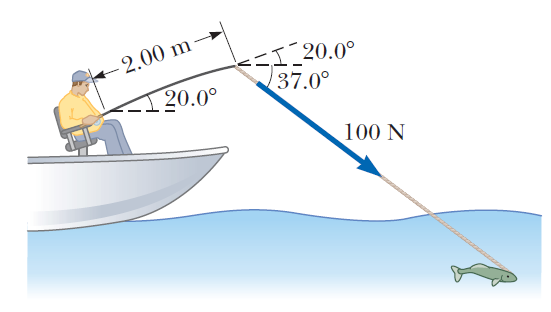
\includegraphics[width=0.6\textwidth]{pez.png}\\
Figura 1. Pescador
\end{center} %Juan Carlos
\item Efectuar el producto cruz entre los vectores
\begin{equation}
u=-\hat{i}+3\hat{k};~ ~~v=2\hat{i}+3\hat{j}+ 9 \hat{k}  
\end{equation} 
%Miguel
% aqui vienen los cuatro ejercicios "dificiles"
\item Problema 10.67 Máquina de Atwood %Miguel
\item Problema 10.87 Un cilindro sólido sobre una mesa. %Juan Carlos
\item Problema 10.95 Un pájaro choca contra un poste. %Juan Carlos
\item Un objeto de masa  $m$  está unido mediante una cuerda a una rueda homogéne a de masa  $M$  y radio  $R$. La cuerda no resbala sobre la rueda y ésta gira sobre su eje sin roce. Encontrar la tensión de la cuerda y la aceleración de la masa.
 \begin{center}
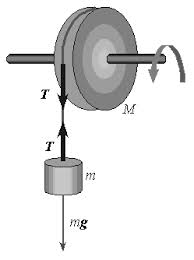
\includegraphics[width=0.6\textwidth]{torque.jpeg}\\
Figura 2. Rueda
\end{center} %Miguel
\end{enumerate}
 

\end{document}


\begin{figure}[h]
\begin{center} 
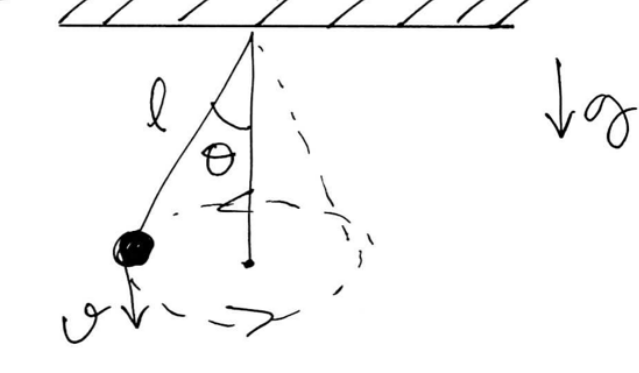
\includegraphics[scale=0.25]{conico.png} 
\caption{\label{fig:conico}Figure para el problema \ref{conico}}
\end{center} 
\end{figure}

\begin{figure}[!h]
\begin{center}
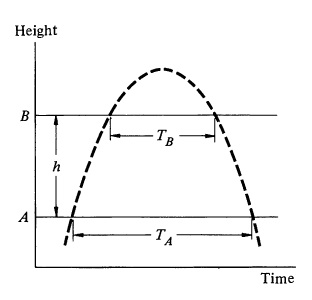
\includegraphics[scale=0.7]{altura.jpg} 
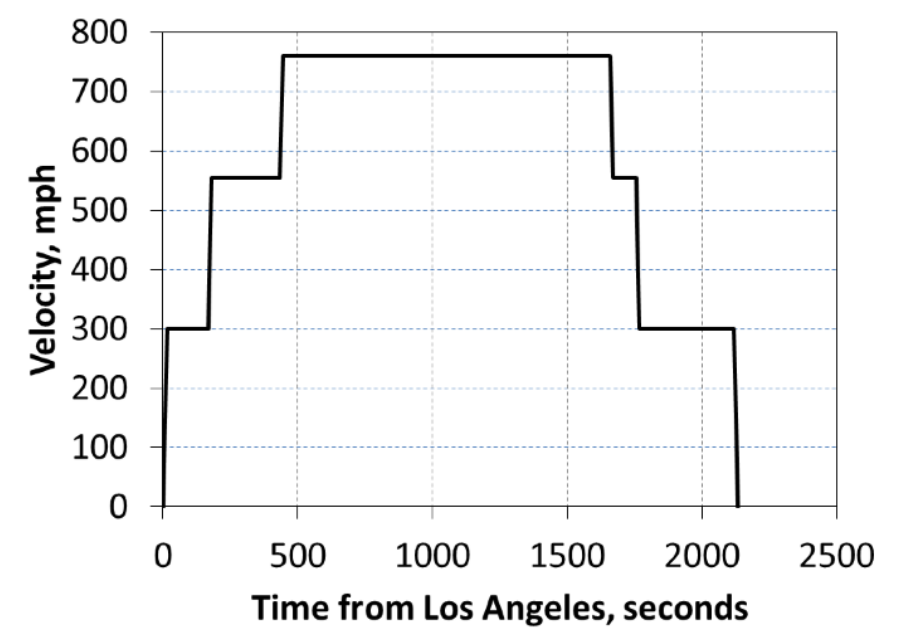
\includegraphics[scale=0.3]{hyperloop.png} 
\end{center}
\caption{Izquierda: diagrama para el ejercicio recomendado 3. Derecha: diagrama para el ejercicio recomendado 4.}
\label{fig:tiro}
\end{figure}





